% !TEX program = xelatex
% =============================================================================
%  Build (identical on Linux and macOS):
%      xelatex template.tex        % twice, for the table of contents
%      latexmk -xelatex template.tex
%
%  Fonts: every font below ships with TeX Live / MacTeX itself and is loaded
%  by *file name* (kpathsea lookup), never by system font name.  That is what
%  makes the same file compile on Linux xelatex and macOS xelatex and produce
%  the same output -- no fontconfig, no Font Book, no font installation.
%  Required TeX Live collections: latex-recommended, fonts-recommended,
%  mathscience (for mathpartir).
% =============================================================================
\documentclass[aspectratio=43]{beamer}

% --- Fonts ------------------------------------------------------------------
% TeX Gyre (Heros = Helvetica, Pagella = Palatino, Cursor = Courier); all three
% live in TeX Live's collection-fontsrecommended and all have real small caps,
% so \textsc{...} keeps working under XeLaTeX.  pdflatex still works through the
% lmodern fallback, so the file never hard-fails on the wrong engine.
\usepackage{iftex}
\ifPDFTeX
  \usepackage[T1]{fontenc}
  \usepackage[utf8]{inputenc}
  \usepackage{lmodern}
\else
  \usepackage{fontspec}
  \defaultfontfeatures{Ligatures=TeX}
  \setsansfont{texgyreheros}[         % beamer typesets slides with this one
    Extension      = .otf,
    UprightFont    = *-regular,
    ItalicFont     = *-italic,
    BoldFont       = *-bold,
    BoldItalicFont = *-bolditalic,
  ]
  \setmainfont{texgyrepagella}[       % only where \rmfamily is asked for
    Extension      = .otf,
    UprightFont    = *-regular,
    ItalicFont     = *-italic,
    BoldFont       = *-bold,
    BoldItalicFont = *-bolditalic,
  ]
  \setmonofont{texgyrecursor}[        % \texttt{...}
    Extension      = .otf,
    UprightFont    = *-regular,
    ItalicFont     = *-italic,
    BoldFont       = *-bold,
    BoldItalicFont = *-bolditalic,
    Scale          = MatchLowercase,
  ]
\fi
% Math stays with beamer's default (Computer Modern): no font file lookup at
% all, so it cannot break on either platform.
%
% ---- Alternative: Computer Modern Sans look (as in Superposition.tex) -------
% Latin Modern has no sans small caps in OpenType form, so \textsc degrades to
% upright text under XeLaTeX -- use it only if the deck has no \textsc:
%   \setsansfont{lmsans10}[Extension=.otf, UprightFont=*-regular,
%     ItalicFont=*-oblique, BoldFont=*-bold, BoldItalicFont=*-boldoblique]
%   \setmainfont{lmroman10}[Extension=.otf, UprightFont=*-regular,
%     ItalicFont=*-italic, BoldFont=*-bold, BoldItalicFont=*-bolditalic]
%   \setmonofont{lmmono10}[Extension=.otf, UprightFont=*-regular,
%     ItalicFont=*-italic, BoldFont=lmmonolt10-bold,
%     BoldItalicFont=lmmonolt10-boldoblique, Scale=MatchLowercase]
%
% ---- Optional: OpenType math.  Needs \documentclass[noamssymb]{beamer} and
%      the amssymb line below removed (unicode-math clashes with amssymb):
%   \usepackage{unicode-math}
%   \setmathfont{texgyrepagella-math.otf}   % or latinmodern-math.otf
%      (texgyrepagella-math is in collection-fontsextra -- install it on both
%       machines with: tlmgr install tex-gyre-math)
%
% ---- Optional: CJK.  No CJK font ships with TeX Live, so name a file that
%      exists on both machines (install Noto CJK on each) rather than a system
%      font name -- "PingFang TC" is macOS-only, "Noto Sans CJK TC" is not:
%   \usepackage{xeCJK}
%   \setCJKmainfont{NotoSerifCJKtc-Regular.otf}
%   \setCJKsansfont{NotoSansCJKtc-Regular.otf}

% --- Packages ---------------------------------------------------------------
\usepackage{xcolor}
\usepackage{colortbl}
\usepackage{graphicx}
\usepackage{amsmath}
\usepackage{amssymb}
\usepackage{mathtools}
\usepackage{mathpartir}   % inference rules -- TeX Live collection-mathscience;
                          % Debian/Ubuntu: apt install texlive-science
\usepackage{hyperref}
\usepackage{fancyvrb}
\usepackage{etoolbox}  % needed for \ifstrequal

% --- Colors -----------------------------------------------------------------
\definecolor{titlecolor}{RGB}{45, 65, 75}    % Dark grey/blue for title
\definecolor{headerbg}{RGB}{35, 50, 55}      % Dark slate grey for header
\definecolor{accentpink}{RGB}{220, 20, 100}  % Pink
\definecolor{accentorange}{RGB}{230, 130, 50}% Orange -- used for emphasis
\definecolor{titleline}{RGB}{245, 225, 210}  % Light peach line
% Dropping the Superposition.tex body in here?  It calls the accents by their
% old names, so add:
%   \colorlet{imandrapink}{accentpink}
%   \colorlet{imandraorange}{accentorange}

% --- Beamer style -----------------------------------------------------------
\setbeamercolor{frametitle}{bg=headerbg, fg=white}
\setbeamercolor{title}{fg=titlecolor}
\setbeamercolor{itemize item}{fg=darkgray}
\setbeamercolor{itemize subitem}{fg=darkgray}

\setbeamertemplate{navigation symbols}{}   % no navigation icons
\setbeamertemplate{footline}{}             % no slide numbers

\setbeamertemplate{title page}{
    \vspace{2.5cm}
    {\usebeamerfont{title}\usebeamercolor[fg]{title}\Large\bfseries \inserttitle}

    \vspace{0.15cm}
    {\small\color{gray} \insertsubtitle}

    \vspace{0.3cm}
    {\color{titleline}\hrule height 1.5pt}
    \vspace{1cm}

    {\small \insertauthor} \\
    \vspace{0.2cm}
    {\small \insertdate}
}

% --- Macros -----------------------------------------------------------------
\newcommand{\Tt}{\mathsf{T}}   % signed-tableau "true"
\newcommand{\Ff}{\mathsf{F}}   % signed-tableau "false"
\newcommand{\hi}[1]{\textcolor{accentorange}{\textbf{#1}}}  % inline highlight

% --- SectionGenerator -------------------------------------------------------
\newbool{skipsectionpage}
\boolfalse{skipsectionpage}

\AtBeginSection[]{
  \ifbool{skipsectionpage}{}{
    \begin{frame}[c]
      \centering
      \vspace{0.8cm}
      {\usebeamercolor[fg]{title}%
       \usebeamerfont{title}%
       \fontsize{20}{30}\selectfont\bfseries
       \insertsection\par}
      \vspace{0.4cm}
      {\usebeamercolor[fg]{structure}\rule{0.35\textwidth}{1.2pt}}
    \end{frame}
  }
}
% --- Presentation meta-data -------------------------------------------------
\title{When Agda met Vampire}
\subtitle{Artjoms \v{S}inkarovs and Michael Rawson}
\author{Jia-Wei Zhang}
\date{08/2026}

\begin{document}

\begin{frame}[plain]
    \titlepage
\end{frame}


% =============================================================================
%  The frames below are the recurring layouts of the deck; keep the ones you
%  need and replace their content.
% =============================================================================
\section{Motivation}
\begin{frame}[t]{Background}
    \vspace{5pt}
    \centering
    \setlength{\tabcolsep}{4pt}%
    \begin{tabular}{|p{0.48\textwidth}|p{0.48\textwidth}|}
      \hline
      \centering\textbf{ATP} & \centering\textbf{ITP} \tabularnewline
      \hline
      \begin{minipage}[t]{\linewidth}\scriptsize\raggedright
        Automated Theorem Proving
        \begin{itemize}\setlength{\itemsep}{1pt}\setlength{\parskip}{0pt}
          \item Machine searches for proof automatically
          \item ATPs are based on Classical FOL
          \item Modern ATPs: \textbf{E}, \textbf{Vampire}
        \end{itemize}
      \end{minipage}
      &
      \begin{minipage}[t]{\linewidth}\scriptsize\raggedright
        Interactive Theorem Proving
        \begin{itemize}\setlength{\itemsep}{1pt}\setlength{\parskip}{0pt}
          \item Human guides proof; machine checks every step
          \item Most ITPs are based on Intuitionistic Logic
          \item Proof Assistants: \textbf{Agda}, \textbf{Rocq}, \textbf{Lean}
        \end{itemize}
      \end{minipage}
      \tabularnewline
      \hline
    \end{tabular}
    \vfill
    Vampire, as the one of state-of-the-art ATP, has been under development for nearly 35 years. \\
    Since 1999, Vampire won 78 titles in CASC.  \\
    Vampire won all competitions in 2025 and 2026!!
\end{frame}

\begin{frame}{Motivation}
    \begin{center}
        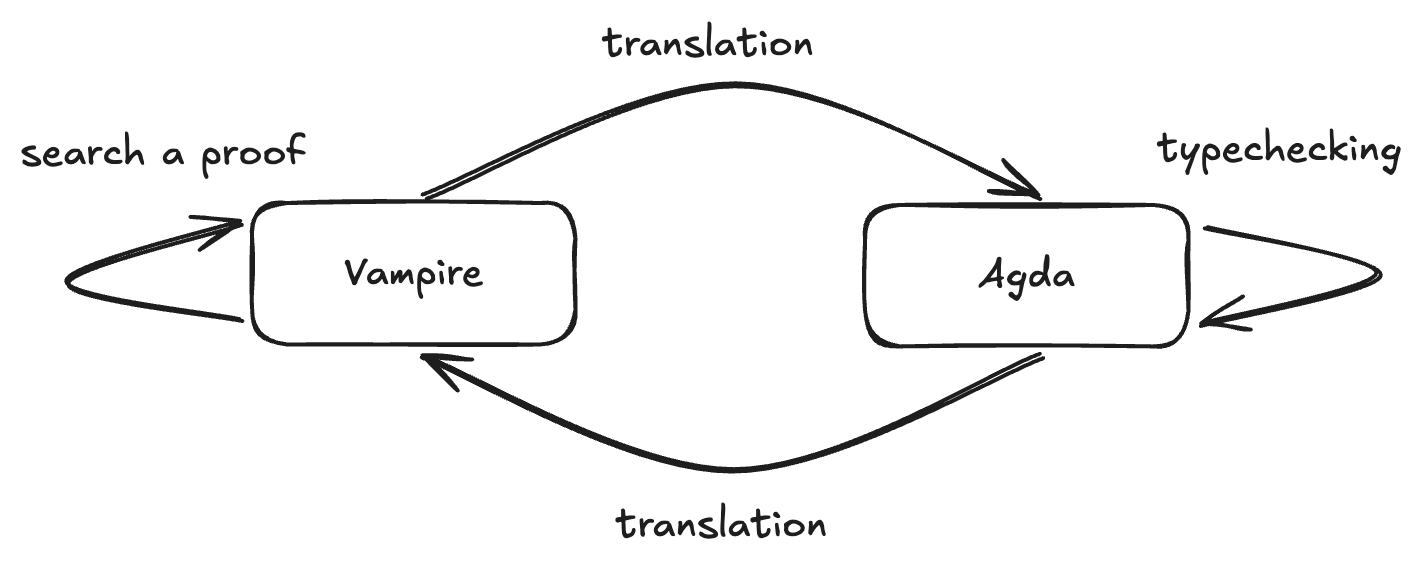
\includegraphics[width=\textwidth,height=0.85\textheight,keepaspectratio]{img/Translation.png}
    \end{center}
\end{frame}

\begin{frame}[fragile]{Example 1: Vector Spaces (without Scalars)}
\begin{Verbatim}[fontsize=\fontsize{5}{6}\selectfont, frame=single, commandchars=\\\{\}]
postulate
  V   : Set                          \textcolor{gray}{-- (declare-sort V 0)}
  ze  : V                            \textcolor{gray}{-- (declare-const ze V)}
  _+_ : V -> V -> V                  \textcolor{gray}{-- (declare-fun _+_ (V V) V)}
  -_  : V -> V                       \textcolor{gray}{-- (declare-fun -_ (V) V)}

  neutl : forall u -> ze + u = u     \textcolor{gray}{-- (assert (! (forall ((u V))}
                                     \textcolor{gray}{--   (= (_+_ ze u) u)) :named neutl))}
  negl  : forall u -> (- u) + u = ze \textcolor{gray}{-- (assert (! (forall ((u V))}
                                     \textcolor{gray}{--   (= (_+_ (-_ u) u) ze))}
                                     \textcolor{gray}{--   :named negl))}
  assoc : forall u v w ->            \textcolor{gray}{-- (assert (! (forall ((u V)(v V)(w V))}
    (u + v) + w = u + (v + w)        \textcolor{gray}{--   (= (_+_ (_+_ u v) w)}
                                     \textcolor{gray}{--      (_+_ u (_+_ v w)))) :named assoc))}
                                     \textcolor{gray}{-- (declare-const u V)}
                                     \textcolor{gray}{-- (declare-const v V)}
ze-uniq' : forall u v ->             \textcolor{gray}{-- (assert (! (forall ()}
  u + v = v -> u = ze                \textcolor{gray}{--   (= (_+_ u v) v)) :named e))}
                                     \textcolor{gray}{-- (assert-not (! (= u ze) :named ze-uniq))}
\end{Verbatim}
Agda to Vampire is based on \textbf{Agda reflection}. \\
\textbf{Agda reflection} is built-in metaprogramming system. \\
\end{frame}

\begin{frame}[fragile]{A Little Taste of Agda}
\begin{Verbatim}[fontsize=\small, frame=single]
trivial : forall u -> -u + (u + u) = u

t1 : -u + (u + u) = (-u + u) + u
t1 = sym (assoc (-u) u u)

t2 : (-u + u) + u = ze + u
t2 = cong (_+ u) (negl u)
   
ans : -u + (u + u) = u
ans = trans t1 t2
\end{Verbatim}
    \vfill
    sym : \{A : Set\} \{x y : A\} x $\equiv$ y $\rightarrow$ y $\equiv$ x \\
    cong : \{A B : Set\} \{x y : A\} (f : A $\rightarrow$ B) $\rightarrow$ x $\equiv$ y $\rightarrow$ f x $\equiv$ f y\\
    trans : \{A : Set\} \{x y z : A\} x $\equiv$ y $\rightarrow$ y $\equiv$ z $\rightarrow$ x $\equiv$ z \\
    negl : \{V : Set\} \{u : V\} (- u) + u = ze \\
    assoc : \{V : Set\} \{u v w : V\} (u + v) + w = u + (v + w) \\
\end{frame}

\begin{frame}{Contents}
    \tableofcontents
\end{frame}

\section{Classical FOL}
\begin{frame}{Classical FOL}
    x y z as individual variable.
    \medskip
    \[
    \begin{array}{r@{\;\;}c@{\;\;}l}
        \mathit{term}    & \Coloneqq & x \mid c \mid f(\mathit{term}, \dots, \mathit{term}) \\[6pt]
        \mathit{atom}    & \Coloneqq & P(\mathit{term}, \dots, \mathit{term})
                                       \mid \mathit{term} = \mathit{term}
                                       \mid \top \mid \bot \\[6pt]
        \mathit{literal} & \Coloneqq & \mathit{atom} \mid \neg\, \mathit{atom} \\[6pt]
        \varphi          & \Coloneqq & \mathit{literal} \mid \neg\varphi \mid \varphi \land \varphi \\[2pt]
                         &           & \mid\ \varphi \to \varphi \mid \varphi \leftrightarrow \varphi \\[2pt]
                         &           & \mid\ \forall x\, \varphi \mid \exists x\, \varphi
    \end{array}
    \]
    The key point of translation: $P \rightarrow Q \equiv \neg P \lor Q$ \\
    Vampire is based on \textbf{refutation proof}. \\
    (It is likely \textbf{proof by contradiction}.) \\
    \vfill
    %-{\footnotesize Vampire draws distinction between \textbf{terms} and \textbf{formulae}. why? \\}
    %-{\footnotesize Terms are inhabitants of the domain, which are \textbf{non-empty}. \\}
    %-{\footnotesize Why non-empty in FOL? \\}
    %-{\footnotesize (Agda x : $\bot$) $\forall x.P(x)$, $\forall x.(P(x) \rightarrow Q)$ $\vdash$ $Q$ \\}
    %-{\footnotesize ($NJ_1$) $\forall$-$E$ would be \textbf{vacuously true} and $\exists$-$I$ would be \textbf{vacuously false.} \\}
\end{frame}

\begin{frame}{Horn Clause and Notation}
    A \textbf{first-order clause} is a \textbf{$\forall$-quantified disjunction of literals}.
    \begin{itemize}
      \item \textbf{Horn clause}: 0 or 1 positive ``head'' literals
      \begin{itemize}
          \item $\forall x y ...$ $L_1 \lor L_2 \lor ...$ 
      \end{itemize}
      \item \textbf{definite clause}: exactly 1 positive literal
      \begin{itemize}
          \item $\forall x y ...$ $\neg A_1 \lor \neg A_2 \lor ... \lor B$ 
          \item $\forall x y ...$ $A_1 \land A_2 \land ... \rightarrow B$
      \end{itemize}
      \item \textbf{goal clause}: exactly 0 positive literals
      \begin{itemize}
          \item $\forall x y ...$ $\neg A_1 \lor \neg A_2 \lor ... \lor \neg A_n$ 
          \item $\forall x y ...$ $A_1 \land A_2 \land ... \land A_n \rightarrow \bot$
      \end{itemize}
    \end{itemize}
    \vfill
    {\footnotesize each $L_i$ are Literal and each $A_i$ and $B$ are Atom. \\}
    {\footnotesize equations s = t are treated as implicitly symmetric. \\}
\end{frame}

\section{Vampire Core Calculus}
%-\begin{frame}[plain]{Vampire framework}
%-    \begin{center}
%-        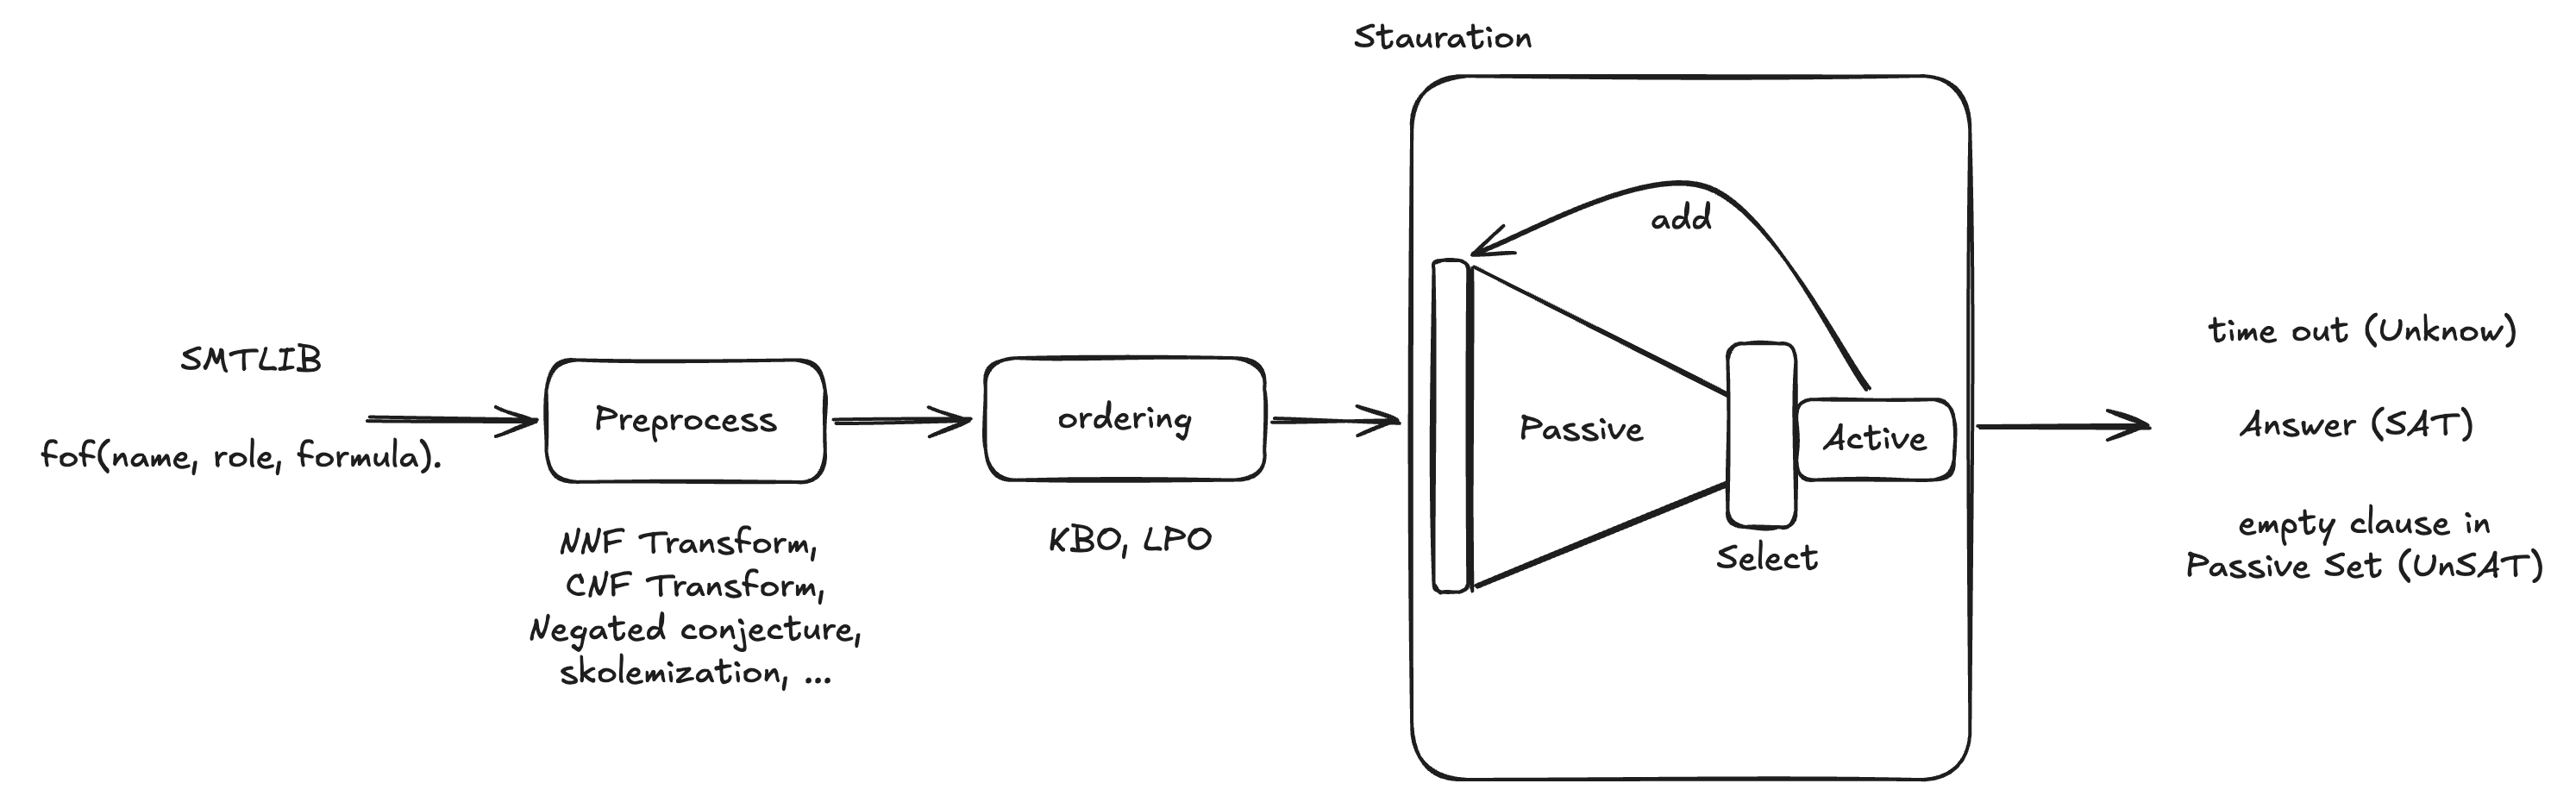
\includegraphics[width=\textwidth,height=\textheight,keepaspectratio]{img/vampire.png}
%-    \end{center}
%-\end{frame}

\begin{frame}{Vampire Core Calculus}
    \begin{mathpar}
        \inferrule*[right=\textsc{Resolution}]{A \lor C \\ \neg A' \lor D}{\sigma(C \lor D)} \and
        \inferrule*[right=\textsc{Factoring}]{A \lor A' \lor C}{\sigma(A \lor C)} \\
        \inferrule*[right=\textsc{Superposition}]{l = r \lor C \\ A[l'] \lor D}{\sigma(A[r] \lor C \lor D)}
        \inferrule*[right=\textsc{Eq.\ Resolution}]{s \neq t \lor C}{\sigma(C)}
    \end{mathpar}
    \vfill
    {\footnotesize $\mathrm{mgu}(A, A')$ in Resolution and Factoring. \\}
    {\footnotesize $\mathrm{mgu}(l, l')$ in Superposition. \\}
    {\footnotesize $\mathrm{mgu}(s, t)$ in Equality Resolution. \\}
    {\footnotesize $A$, $A[l']$ are atoms. \\}
    {\footnotesize $C$, $D$ are clauses. \\}
    {\footnotesize $l$, $l'$, $r$, $s$, $t$ are terms. \\}
\end{frame}

%-\begin{frame}{Superposition derived from Resolution}
%-    \begin{columns}
%-        \begin{column}{0.4\textwidth}
%-            \centering
%-            $\inferrule*[right=\textsc{BR}]{A \lor C_1 \\ \neg A \lor C_2}{C_1 \lor C_2}$
%-        \end{column}
%-        \begin{column}{0.55\textwidth}
%-            \centering
%-            $\inferrule*[right=\textsc{ER}]{
%-                \inferrule*[right=\textsc{Sup}]
%-                    {A = \top \lor C_1 $\space$ A \neq \top \lor C_2}
%-                    {\top \neq \top \lor C_1 \lor C_2}
%-            }{C_1 \lor C_2}$
%-        \end{column}
%-    \end{columns}
%-    \vfill
%-\end{frame}

\begin{frame}[fragile]{Example 1 (Vector Spaces)}
\begin{Verbatim}[fontsize=\fontsize{5}{6}\selectfont, frame=single, commandchars=\\\{\}]
 1. forall x. 0 + x = x  (neutl)
 2. forall x. (-x) + x = 0  (negl)
 3. forall xyz. (x+y)+z = x+(y+z)  (assoc)
 4. v = u + v  (e)
 5. 0 != u  (negated goal)
 6. forall xy. -x+(x+y) = 0+y  (superposition 3, 2)
 7. forall x. v+x = u+(v+x)  (superposition 3, 4)
 8. forall xy. -x+(x+y) = y  (superposition 6, 1)
 9. forall x. (--x)+0 = x  (superposition 8, 2)
10. forall xy. y+x = (--y)+x  (superposition 8, 8)
11. forall x. x+0 = x  (superposition 9, 10)
12. forall x. 0 = x+(-x)  (superposition 2, 10)
13. 0 = u+0  (superposition 7, 12)
14. 0 = u  (superposition 13, 11)
15. false  (resolution 14, 5)

\textcolor{gray}{-- Vampire Original Output}
\textcolor{gray}{ 1. 'vec._+_'('vec.ze',X0) = X0}
\textcolor{gray}{ 2. 'vec._+_'('vec.-_'(X0),X0) = 'vec.ze'}
\textcolor{gray}{ 3. 'vec._+_'('vec._+_'(X0,X1),X2) = 'vec._+_'(X0,'vec._+_'(X1,X2))}
\textcolor{gray}{ 4. v = 'vec._+_'(u,v)}
\textcolor{gray}{ 5. 'vec.ze' != u}
\textcolor{gray}{ 6. 'vec._+_'('vec.-_'(X0),'vec._+_'(X0,X1)) = 'vec._+_'('vec.ze',X1)}
\textcolor{gray}{ 7. 'vec._+_'(v,X0) = 'vec._+_'(u,'vec._+_'(v,X0))}
\textcolor{gray}{ 8. 'vec._+_'('vec.-_'(X0),'vec._+_'(X0,X1)) = X1}
\textcolor{gray}{ 9. 'vec._+_'('vec.-_'('vec.-_'(X0)),'vec.ze') = X0}
\textcolor{gray}{10. 'vec._+_'(X1,X0) = 'vec._+_'('vec.-_'('vec.-_'(X1)),X0)}
\textcolor{gray}{11. 'vec._+_'(X0,'vec.ze') = X0}
\textcolor{gray}{12. 'vec.ze' = 'vec._+_'(X0,'vec.-_'(X0))}
\textcolor{gray}{13. 'vec.ze' = 'vec._+_'(u,'vec.ze')}
\textcolor{gray}{14. 'vec.ze' = u}
\textcolor{gray}{15. $false}
\end{Verbatim}
\end{frame}

\begin{frame}{Example 1 (Vector Spaces)}
    \footnotesize
    \begin{center}
    $\begin{array}{r@{\quad}l@{\qquad}l}
      2 & \forall x.\; (-x) + x = 0                  & (l = r)\\[3pt]
      3 & \forall x\,y\,z.\; (x+y)+z = x+(y+z)       & (A[l'])
    \end{array}$
    \end{center}
    \vspace{4pt}
    \textbf{Sup 3, 2}
    \begin{mathpar}
      \inferrule*[right=\textsc{Sup}]{l = r \\ A[l']}{\sigma(A[r])}
    \end{mathpar}
    \textbf{\[\sigma = \{\, x \mapsto -x,\; y \mapsto x \,\}\]}
    \begin{mathpar}
      \inferrule*[right=\textsc{Sup}]{(-x) + x = 0 \\ ((-x) + x) + z = (-x) + (x + z)}{0 + z = (-x) + (x + z)}
    \end{mathpar}
\end{frame}

\section{Vampire to Agda}
\begin{frame}{A classical proof to intuitionistic proof}
    Restricting both systems to a common language (Horn Clause). \\
    They wish to show $\Gamma \vdash G$, and Vampire obtain a classical proof by refutation showing $\Gamma, \neg G \vdash \bot$
    \begin{itemize}
        \item $\Gamma, \neg G \vdash \bot$ 
        \item $\Gamma, G \rightarrow \bot \vdash \bot$ 
        \item $\Gamma, G \rightarrow G \vdash G$ (replacing occurrences of $\bot$ with G)
    \end{itemize}
    \vfill
    {\footnotesize $\Gamma$ is a set of definite clauses, $G$ is "ground goal atom". \\}
    {\footnotesize In general $\bot$ may be woven through the entire proof, \\}
    {\footnotesize replacing $\bot$ from top right of tree. \\}
\end{frame}

\begin{frame}{Lemmas}
    \begin{itemize}
        \item Lemma 1: If Premises are Horn clause, then Conclusion is also Horn.
        \item Lemma 2: Horn Vampire Core Calculus(HVCC) is intuitionistically valid.
        \item Lemma 3 (Redundancy Property) : If we finally derived  $\bot$ from Horn Vampire Core Calculus(HVCC), then ???
    \end{itemize}
    \vfill
    {\footnotesize Vampire Core Calculus = VCC, Horn VCC = HVCC \\}
\end{frame}

\begin{frame}{Vampire Core Calculus (General and Horn Clause)}
    \tiny
    \begin{columns}[T]
      \begin{column}{0.46\textwidth}
        \centering\scriptsize\textbf{VCC}
        \begin{mathpar}
          \inferrule*[right=\textsc{Res.}]{A \lor C \quad \neg A' \lor D}{\sigma(C \lor D)}
        \end{mathpar}
        \vspace{2pt}
        \begin{mathpar}
          \inferrule*[right=\textsc{Fac.}]{A \lor A' \lor C}{\sigma(A \lor C)}
        \end{mathpar}
        \vspace{2pt}
        \begin{mathpar}
          \inferrule*[right=\textsc{Eq.Res.}]{s \neq t \lor C}{\sigma(C)}
        \end{mathpar}
        \vfill
        \begin{mathpar}
          \inferrule*[right=\textsc{Sup.}]{l = r \lor C \quad A[l'] \lor D}{\sigma(A[r] \lor C \lor D)}
        \end{mathpar}
      \end{column}
      \begin{column}{0.54\textwidth}
        \centering\scriptsize\textbf{HVCC}
        \begin{mathpar}
          \inferrule*[right=\textsc{Res.}]{\neg P \lor A \quad \neg A' \lor \neg Q \lor \boxed{B}}{\sigma(\neg P \lor \neg Q \lor \boxed{B})}
        \end{mathpar}
        \begin{mathpar}
          \inferrule*[right=\textsc{Fac.}]{\neg A \lor \neg A' \lor \neg P \lor \boxed{B}}{\sigma(\neg A \lor \neg P \lor \boxed{B})}
        \end{mathpar}
        \begin{mathpar}
          \inferrule*[right=\textsc{Eq.Res.}]{s \neq t \lor \neg P \lor \boxed{A}}{\sigma(\neg P \lor \boxed{A})}
        \end{mathpar}
        \begin{mathpar}
          \inferrule*[right=\textsc{Sup.L}]{\neg P \lor l = r \quad \neg A[l'] \lor \neg Q \lor \boxed{B}}{\sigma(\neg P \lor \neg A[r] \lor \neg Q \lor \boxed{B})}
        \end{mathpar}
        \begin{mathpar}
          \inferrule*[right=\textsc{Sup.R}]{\neg P \lor l = r \quad \neg Q \lor A[l']}{\sigma(\neg P \lor \neg Q \lor A[r])}
        \end{mathpar}
      \end{column}
    \end{columns}
    \vfill
    {\footnotesize P, Q = premises;\; A, B = atoms;\; C, D = clauses;\; \\
     $\mathrm{mgu}(A,A')$, $\mathrm{mgu}(l,l')$, $\mathrm{mgu}(s,t)$ \\ }
    {\footnotesize $\boxed{}$ = positive atom. \\}
    {\footnotesize $\neg$P = $\neg(A_1 \land A_2 ...)$, C = $\neg A_1 \lor \neg A_2 ...$ (Horn and De Morgan) \\}
\end{frame}

\begin{frame}{Vampire Core Calculus (Clause and Implication)}
    \tiny
    \begin{columns}[T]
      \begin{column}{0.50\textwidth}
        \centering\scriptsize\textbf{HVCC}
        \begin{mathpar}
          \inferrule*[right=\textsc{Res.}]{\neg P \lor A \quad \neg A' \lor \neg Q \lor \boxed{B}}{\sigma(\neg P \lor \neg Q \lor \boxed{B})}
        \end{mathpar}
        \begin{mathpar}
          \inferrule*[right=\textsc{Fac.}]{\neg A \lor \neg A' \lor \neg P \lor \boxed{B}}{\sigma(\neg A \lor \neg P \lor \boxed{B})}
        \end{mathpar}
        \begin{mathpar}
          \inferrule*[right=\textsc{Eq.Res.}]{s \neq t \lor \neg P \lor \boxed{A}}{\sigma(\neg P \lor \boxed{A})}
        \end{mathpar}
        \begin{mathpar}
          \inferrule*[right=\textsc{Sup.L}]{\neg P \lor l = r \quad \neg A[l'] \lor \neg Q \lor \boxed{B}}{\sigma(\neg P \lor \neg A[r] \lor \neg Q \lor \boxed{B})}
        \end{mathpar}
        \begin{mathpar}
          \inferrule*[right=\textsc{Sup.R}]{\neg P \lor l = r \quad \neg Q \lor A[l']}{\sigma(\neg P \lor \neg Q \lor A[r])}
        \end{mathpar}
      \end{column}
      \begin{column}{0.50\textwidth}
        \centering\scriptsize\textbf{HVCC$^{Imp}$}
        \begin{mathpar}
          \inferrule*[right=\textsc{Res.}]{P \to A \quad A' \land Q \to \boxed{B}}{\sigma(P \land Q \to \boxed{B})}
        \end{mathpar}
        \begin{mathpar}
          \inferrule*[right=\textsc{Fac.}]{A \land A' \land P \to \boxed{B}}{\sigma(A \land P \to \boxed{B})}
        \end{mathpar}
        \begin{mathpar}
          \inferrule*[right=\textsc{Eq.Res.}]{s = t \land P \to \boxed{A}}{\sigma(P \to \boxed{A})}
        \end{mathpar}
        \begin{mathpar}
          \inferrule*[right=\textsc{Sup.L}]{P \to l = r \quad A[l'] \land Q \to \boxed{B}}{\sigma(P \land A[r] \land Q \to \boxed{B})}
        \end{mathpar}
        \begin{mathpar}
          \inferrule*[right=\textsc{Sup.R}]{P \to l = r \quad Q \to A[l']}{\sigma(P \land Q \to A[r])}
        \end{mathpar}
      \end{column}
    \end{columns}
    \vfill
    {\footnotesize P, Q = premises;\; A, B = atoms;\;
     $\mathrm{mgu}(A,A')$, $\mathrm{mgu}(l,l')$, $\mathrm{mgu}(s,t)$.}
\end{frame}

\begin{frame}{Vampire Core Calculus (Propositions as types)}
    \tiny
    \begin{columns}[T]
      \begin{column}{0.46\textwidth}
        \centering\scriptsize\textbf{HVCC$^{Imp}$}
        \begin{mathpar}
          \inferrule*[right=\textsc{Res.}]{P \to A \quad A' \land Q \to \boxed{B}}{\sigma(P \land Q \to \boxed{B})}
        \end{mathpar}
        \begin{mathpar}
          \inferrule*[right=\textsc{Fac.}]{A \land A' \land P \to \boxed{B}}{\sigma(A \land P \to \boxed{B})}
        \end{mathpar}
        \begin{mathpar}
          \inferrule*[right=\textsc{Eq.Res.}]{s = t \land P \to \boxed{A}}{\sigma(P \to \boxed{A})}
        \end{mathpar}
        \begin{mathpar}
          \inferrule*[right=\textsc{Sup.L}]{P \to l = r \quad A[l'] \land Q \to \boxed{B}}{\sigma(P \land A[r] \land Q \to \boxed{B})}
        \end{mathpar}
        \begin{mathpar}
          \inferrule*[right=\textsc{Sup.R}]{P \to l = r \quad Q \to A[l']}{\sigma(P \land Q \to A[r])}
        \end{mathpar}
      \end{column}
      \begin{column}{0.54\textwidth}
        \centering\scriptsize\textbf{Agda}
        \begin{mathpar}
          \inferrule*[right=\textsc{Res.}]{t_1 : P \to A \quad t_2 : A \land Q \to B}{(\lambda (p,q).\; t_2\; (t_1\; p, q)) : P \land Q \to B}
        \end{mathpar}
        \vspace{2pt}
        \begin{mathpar}
          \inferrule*[right=\textsc{Fac.}]{t : A \land A \land P \to B}{(\lambda (a,p).\; t\; (a, a, p)) : A \land P \to B}
        \end{mathpar}
        \vspace{1.5pt}
        \begin{mathpar}
          \inferrule*[right=\textsc{Eq.Res.}]{t : s = s \land P \to A}{(\lambda p.\; t\; \mathsf{refl}\; p) : P \to A}
        \end{mathpar}
        \begin{mathpar}
          \inferrule*[right=\textsc{Sup.L}]{t_1 : P \to l = r \quad t_2 : A[l] \land Q \to B}{(\lambda (p,a,q).\; t_2\; ((\mathsf{subst}\; (\mathsf{sym}\; (t_1\; p))\; a), q)) \\\\ : P \land A[r] \land Q \to B}
        \end{mathpar}
        \begin{mathpar}
          \inferrule*[right=\textsc{Sup.R}]{t_1 : P \to l = r \quad t_2 : Q \to A[l]}{(\lambda pq.\; \mathsf{subst}\; (t_1\; p)\; (t_2\; q)) : P \land Q \to A[r]}
        \end{mathpar}
      \end{column}
    \end{columns}
    \vfill
    {\footnotesize $\mathsf{subst} : l = r \to A[l] \to A[r]$,
     $\mathsf{sym} : l = r \to r = l$. \\ }
\end{frame}

%-\begin{frame}{Superposition derived from Resolution (Cont)}
%-    \begin{mathpar}
%-        \inferrule*[right=\textsc{Sup.L}]{l = r \lor C \\ A[l] \neq t \lor D}{\sigma(A[r] \neq t \lor C \lor D)}
%-        \inferrule*[right=\textsc{Sup.R}]{l = r \lor C \\ A[l] = t \lor D}{\sigma(A[r] = t \lor C \lor D)}
%-    \end{mathpar}
%-    \vfill
%-    {\footnotesize Ordering conditions:
%-    \begin{enumerate}
%-        \item $l \succ r$
%-        \item $A[l] \succ t$
%-        \item $l = r$ is strictly greater than any literal in $C$
%-        \item (superposition-right only) $A[l] = t$ is greater than or equal to any literal in $D$
%-    \end{enumerate}
%-    }
%-\end{frame}

\begin{frame}{Example 2}
    \footnotesize
    \begin{center}
    $t_1\!:\!\forall x.\, f(x) = x,\;\;
     t_2\!:\! a = f(c),\;\;
     t_3\!:\! b = c,\;\;
     t_4\!:\! a = b \to \boxed{\bot}
     \;\;\vdash\; \boxed{\bot}$
    \end{center}
    \vfill
    \scriptsize
    \begin{mathpar}
      \inferrule*[right=\textsc{Eq.Res.}]{
        \inferrule*[right=\textsc{Sup.L}]{
          b = c
          \inferrule*[right=\textsc{Sup.L}]{
            f(c) = c
            \\
            \inferrule*[right=\textsc{Sup.L}]{a = f(c) \\ a = b \to \boxed{\bot}}{f(c) = b \to \boxed{\bot}}
          }{c = b \to \boxed{\bot}}
        }{c = c \to \boxed{\bot}}
      }{\boxed{\bot}}
    \end{mathpar}
    {\footnotesize replace each $\boxed{\bot}$ by a = b}
\end{frame}

\section{Thesis Proposal}
\begin{frame}{Thesis Proposal}
    \begin{itemize}
        \item Formalize HVCC$^{Imp}$ (5 Implication rules) by deep embedding.
        \item Prove the $\Gamma, G \rightarrow \bot \vdash \bot$, replace $\bot$ by $G$. \\
        (Lemma1, 2, 3) \\
    \end{itemize}
\end{frame}

\booltrue{skipsectionpage} % skip central title
\section{References}
\begin{frame}{References}
    \scriptsize
    \begin{itemize}
        \item Artjoms Šinkarovs and Michael Rawson. ``When Agda Met Vampire.''
        \item Laura Kovács and Andrei Voronkov.  "Vampire Guide Lectures."
        \item Giles Reger. "The Vampire Journey. (Youtube)"
        \item Alan J.A. Robinson, Andrei Voronkov. "Paramodulation-Based Theorem Proving"
    \end{itemize}
\end{frame}

\end{document}
